\documentclass[12pt]{article}
\usepackage[T2A]{fontenc}
\usepackage[utf8]{inputenc}
\usepackage[russian, english]{babel}
\usepackage{graphicx}
\usepackage{amssymb}
\usepackage{amsmath}
\usepackage{mathrsfs}
\usepackage[left=2cm,right=2cm, top=2cm,bottom=2cm,bindingoffset=0cm]{geometry}
\author{Георгий Баронча, 726 группа}
\title{\textbf{Лабораторная работа 4.3.1 }\\				
Изучение дифракции света}
\date{20 марта 2019}
\begin{document}
	\maketitle
	\subsection{Цель работы}
	 Исследовать явления дифракции Френеля и Фраунгофера на щели, изучить влияние дифракции на разрешающую способность оптических инструментов.
	\subsection{Приборы и материалы}
	Оптическая скамья, ртутная лампа, монохроматор, щели с регулируемой шириной, рамка с вертикальной нитью, двойная щель, микроскоп на поперечных салазках с микрометрическим винтом.
\section{Дифракция Френеля}
\subsection{Немного теории}
	 Пусть сферическая волна распространяется в пространстве(рис. 1).
	 \begin{figure}[h]
	 	\centering	
	 	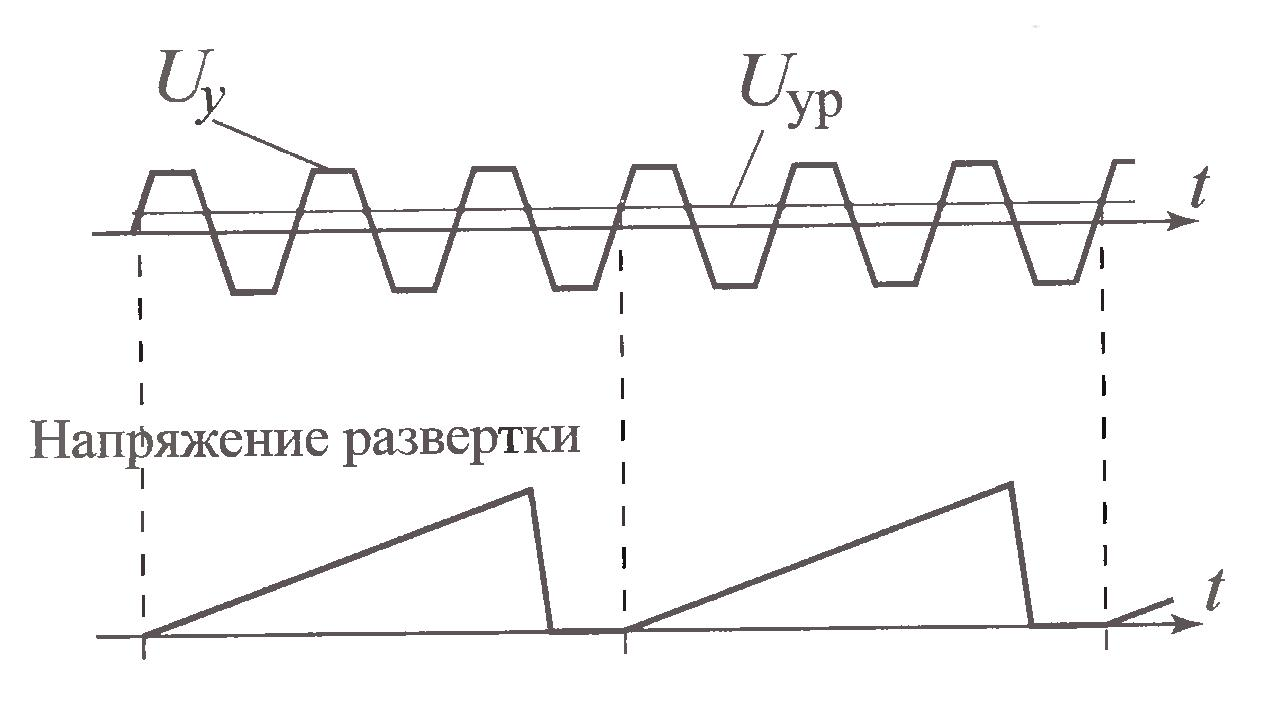
\includegraphics[width=0.6\textwidth]{pic2.jpg}
	 	\caption{распространение сферической волны}
	 \end{figure}\\
	 
	  Тогда её амплитуда в точке $P$ выражается с помощью формулы (1):
	 \begin{equation}
	 E_0(P) = \frac{E_0 e^{ika}}{a} \iint\limits_\sigma k(\psi) \frac{e^{ikr}}{r}\,d\sigma.
	 \end{equation} 
	 Тоесть, мы разбиваем на окружности(в силу симметрии) толщиной $d\sigma$ и подсчитываем их вклад в общую напряженность.\\
	 Френель предложил разбить волновую поверхность на зоны, так чтобы $k(\psi)$ стало числом $k_n$, не зависящим от $\psi$ в пределах одной зоны: \begin{equation}
	 r_1 = b + \lambda/2, \mbox{ }\mbox{ }\mbox{ } r_2 = b + \lambda,...
	 \end{equation}
	 В общем случае радиус $n$-ой зоны: \begin{equation}
	 r_n = \sqrt{n \frac{ab}{a+b}\lambda}
	 \end{equation}
	 Колебания, возбуждаемые в точке $P$ между двумя соседними зонами, противоположны по фазе, так как разность хода от этих зон до точки P равна $\Delta = \lambda/2$.\\
	 С учетом того, что площади соседних зон примерно равны, можно найти сумму: \begin{equation}
	 S_n = k_1 + k_2 + \dots + k_n = \frac{k_1}{2} + (\frac{k_1}{2} - k_2 + \frac{k_3}{2}) + \dots = (k_1 \pm k_n)/2
	 \end{equation}
	 Откуда сразу получается: \begin{equation}
	 E_0(P) = \frac{1}{2}E_{01} + \frac{1}{2}E_{0n}
	 	 \end{equation}
	 Заметим, что $k(\pi/2) = 0$, следовательно при $n \rightarrow \infty$ напряжение $E_0(P) \rightarrow \frac{1}{2}E_{01}$. Интенсивность $I \sim E^2 \Rightarrow I_0 = I_1/4$. Таким образом, результирующая интенсивность, создаваемая в точке $P$ всей сферической поверхностью равна четверти интенсивности, создаваемой одной центральной зоной.\\
	 Для характеристики наблюдаемой картины вводят волновой параметр $p$: \[
	 	p = \frac{\sqrt{z\lambda}}{b}
	 \]
	 \begin{itemize}
	 	\item  При $p \ll 1$ дифракционная картина отсутствует, а распределение интенсвиностей вычисляется с помощью законов геометрической оптики.
	 	\item При $p \simeq 1$ наблюдается дифракция Френеля.
	 	\item  При  $p \gg 1$ наблюдается дифракция Фраунгофера.
	 \end{itemize}
 \newpage
	 \subsection{Экспериментальная установка}
	 Схема экспериментальной установки приведена на рисунке 2.
	  \begin{figure}[h]
	 	\centering	
	 	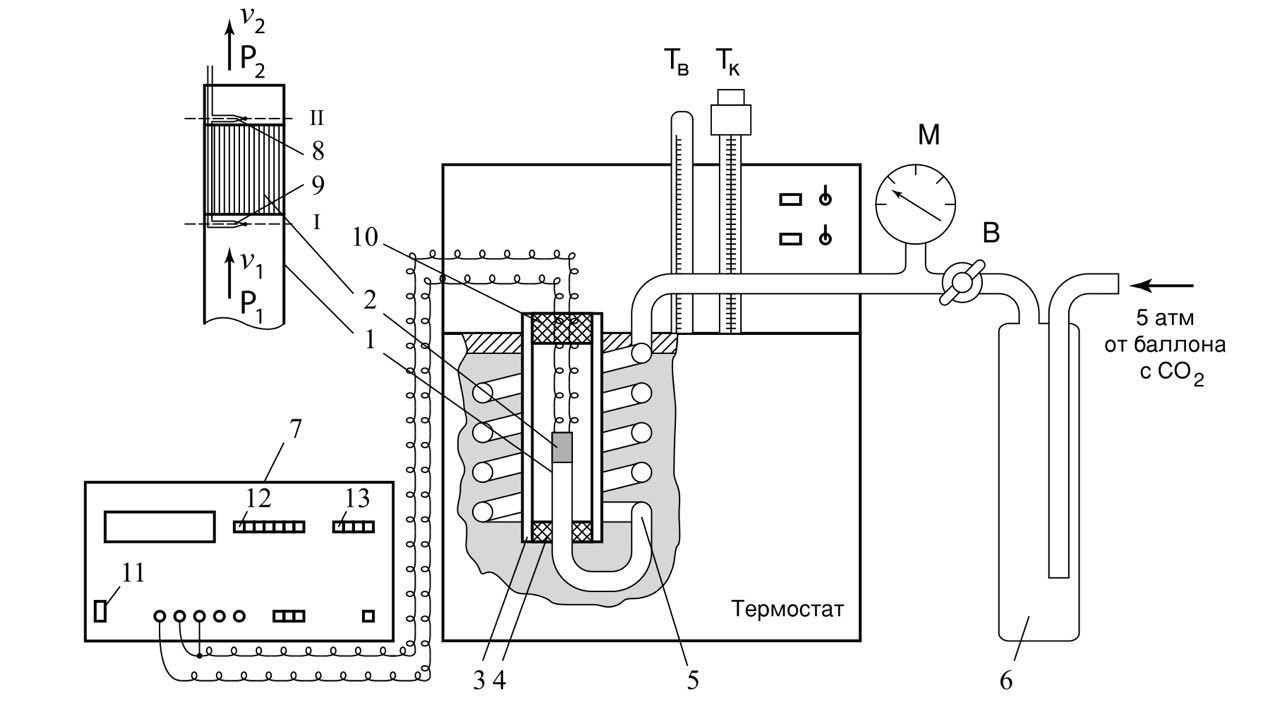
\includegraphics[width=0.9\textwidth]{pic1.jpg}
	 	\caption{схема установки}
	 \end{figure}\\
 
Световые лучи освещают щель $S_2$ и испытывают на ней дифракцию. Дифракционная картина рассматривается с помощью микроскопа $M$, сфокусированного на некоторую плоскость наблюдения П. \\
С другой стороны, ртутная лампа Л светит на монохроматор С, откуда спектральная линия фокусируется на щель $S_1$, проходит через объектив $O_1$ и попадает на вышеупомянутую щель $S_2$.\\
	Монохроматор работает на принципе дисперсии света. Свет проходит через узкую щель, а далее отражается от диспергирующего элемента, а нужная часть спектра фокусируется на узкой щели. Схема монохроматора представлена на рисунке 3. 
	 \begin{figure}[h]
		\centering	
		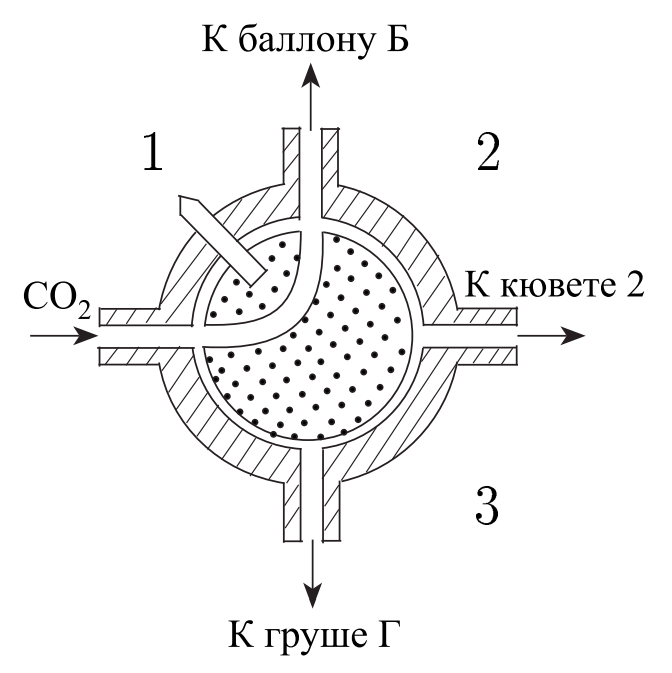
\includegraphics[width=0.5\textwidth]{pic3.png}
		\caption{схема монохроматора Черни-Тёрнера}
	\end{figure}\\
	В качестве диспергирующего элемента в нашей установке использовалась призма. Для стекла ТФ-1 дисперсия показателя преломления: \[
	\frac{dn}{d\lambda} \approx -1,17 \cdot 10^3 \mbox{ см}^{-1}
	\]
	При изменении коэффициента преломления меняется и коэффициент отражения, а значит различные цвета проходят различный оптический путь, что приводит к возникновению разности хода двух лучей. Так, после прохождения призмы "фиолетовые" лучи отклоняются больше, чем "красные".\\
	Закон дисперсии $n(\lambda)$ приведен на рисунке 4. 
		  \begin{figure}[h]
		\centering	
		\includegraphics[width=0.45\textwidth]{pic4.jpg}
		\caption{качественная зависимость $n(\lambda)$}
	\end{figure}\\
	В области между $\lambda_n$ и $\lambda_m$ показатель преломления растет с длиной волны -- это так называемая область аномальной дисперсии. Аномальная дисперсия имеет место на частотах, близких к резонансным, и соответственно в этой области велико поглащение света. Стекло в оптическом диапазоне длин волн имеет нормальную дисперсия, а аномальная наблюдается лишь в \\ ультрафиолетовой области спектра.\\
	\subsection{Ход работы}
	Измеренная ширина щели:
	\begin{itemize}
		\item согласно микрометрическому винту щели $b = 0,345 \pm 0,005$ мм.
		\item согласно микрометрическому винту микроскопа $b = 0,32 \pm 0,03$ мм.
	\end{itemize}
	Приближая микроскоп к щели, снимем зависимость координаты микроскопа от числа $n$ темных полос по формуле $z_n = x_0 - x_n$, где $x_0 = 55,4$ мм -- положение нуля, $x_n$ -- координата микроскопа, когда видно $n$ темных полос.\\
	Длина зеленого света $\lambda = 5461 \cdot 10^{-10}$ м.\\
	Погрешность $2\xi_n$ рассчитаем по формуле: \begin{equation}
	\delta(2\xi_n) = \frac{\delta z}{2z}(2\xi_n) 
	\end{equation}
	\newpage
	Результаты измерений занесены в таблицу.\\
	\begin{table}[h!]
		\begin{tabular}{||c|c|c|c|c|c||c||l|l||l|l|}
			\hline
			
			\hline
			количество полос $m$ & $x$, см&  $\delta z$, см  &  $2\delta\xi_n$, мм & $2\xi_n$, мм & $\delta(2\xi_n)$, мм \\
			\hline
			1 & 52,6 & 0,2 & 2,8 & 0,350 & 0,01 \\
			2 & 53,5 & 0,2 & 1,9 & 0,353 & 0,02\\
			3 & 54,1 & 0,2 & 1,3 & 0,337 & 0,03\\
			4 & 54,4 & 0,2 & 1,0 & 0,330 & 0,03\\
			5 & 54,5 & 0,2 & 0,9 & 0,343 & 0,04\\
			\hline
		\end{tabular}
		\caption{Экспериментальных данные: зависимость координаты микроскопа от числа $n$ темных полос}
	\end{table}
	\\
	Среднее значение $2\xi_n = (0,341 \pm 0,005)$ мм.\\
	По данным таблицы 1 строю график зависимости  суммарной ширины зон Френеля от их числа $2\xi_n(n)$. \\
	Исходя из графика делаем заключение, как и ожидалось, ширина зон совпадает с шириной щели.
	\section{Дифракция Фраунгофера на щели} 
	\subsection{Немного теории}
	При падении световой волны на щель возникает разность хода, как показано на рисунке 5.\\
		  \begin{figure}[h]
		\centering	
		\includegraphics[width=0.7\textwidth]{pic5.jpg}
		\caption{возникновение разности хода}
	\end{figure}\\
Разность хода: \[
 	\Delta = x\sin \theta
\]
Тогда: \begin{equation}
dE_{\theta} = E_0 \frac{dx}{b} e^{ikx\sin\theta}
\end{equation}
Интегрируя (7):
\begin{equation}
E_{\theta} = \frac{E_0}{b} \int\limits_{-b/2}^{b/2} e^{ikx\sin\theta} \,dx = \frac{E_0 \sin u}{u}, \mbox{ }\mbox{ }\mbox{ где } u= \frac{kb}{2}\sin \theta 
\end{equation}
С учетом того, что $I \sim E^2$, получим: \begin{equation}
I(\sin \theta) = I_0 \Bigl(\frac{\sin u}{u}\Bigl)^2
\end{equation}
Минимум достигается: \begin{equation}
u = \frac{kb}{2}\sin \theta = \frac{\pi b \sin \theta}{\lambda} = m\pi \mbox{ } \Rightarrow  \mbox{ }\sin \theta_{\min} = \frac{m\lambda}{b}
\end{equation}
\subsection{Экспериментальная установка}
	Дифракцию Френеля и Фраунгофера можно наблюдать на одной и той же установке, однако при обычных размерах установки дифракция Фраунгофера возникает только при очень узких щелях. Поэтому в схеме установки для дифракции Френеля для наблюдения дифракции Фраунгофера добавляется объектив $O_2$ между щелью $S_2$ и плоскостью П.\\
	Дифракционная картина наблюдается здесь в фокальной плоскости $O_2$. Каждому значению угла $\theta$ соответствует в этой плоскости точка, отстоящая от оси на расстоянии \begin{equation}
	x = f_2\tan \theta \approx f_2 \theta
	\end{equation}
	В центре поля зрения наблюдается дифракционный максимум(светлая полоса). При малых углах $\theta$ положение минимумов определяется соотношением(10).\\
	Расстояние $x_m$ от темной полосы до оптической оси объектива $O_2$ пропорционально фокусному расстоянию $f_2$. Следовательно: \begin{equation}
	x_m = m\frac{\lambda}{b}f_2
	\end{equation}
	Видно, что при малых углах минимумы эквидистантны, а расстояние между минимумами обратно пропорционально ширине щели $S_2$.
	\subsection{Ход работы}
	Величина щели по винту равна $b = 0,165 \pm 0,005$ мм. Фокусное расстояние линзы $f_2 = 12,5$ см. Фокусное растояние линзы $f_1 = 10,0$ см.\\
	Измерим с помощью винта поперечного перемещения микроскопа координаты $X_m$ нескольких дифракционных минимумов (3 слева от максимума, и три справа). Здесь $x_m$ -- показания микрометрического винта, которые затем умножаем на $\alpha = 0,01$ мм -- цену деления винта, т.е. $X_m = \alpha x_m$.\newpage Результаты занесем в табл. 2 и построим график зависимости минимумов от их номеров.

	\begin{table}[h!]
		\begin{tabular}{||c|c|c|c|c||c||c||l|l||l|l|}
			\hline
			
			\hline
			количество полос $m$ & $x_m$, см&  $\delta x_m$, см  &  $X_m$, мм & $\delta X_m$, мм \\
			\hline
			1 & 0,0 & 0,5 & 0 & 0,005 \\
			2 & 4,2 & 0,5 & 0,042 & 0,005 \\
			3 & 9,1 & 0,5 & 0,091 & 0,005 \\
			4 & 14,1 & 0,5 & 0,141 & 0,005 \\
			5 & 20,1 & 0,5 & 0,201 & 0,005 \\
			6 & 25,6 & 0,5 & 0,256 & 0,005\\
			7 & 30,1 & 0,5 & 0,301 & 0,005\\
			\hline
		\end{tabular}
		\caption{Зависимость положения темных полос от их номера $m$ при дифракции Фраунгофера на одной щели}
	\end{table}
	Из графика получаем, что угол наклона $a = (5,2 \pm 0,1) \cdot 10^{-2}$ мм. Это и есть расстояние $\Delta X$ между соседними максимумами. Из формулы (12) мы получаем, что \begin{equation}
	b_e = \frac{\lambda f_2}{\Delta X} = 0,134 \mbox{ мм}
	\end{equation}
	Погрешность $b_e$:
	\begin{equation}
	\delta b_e = \frac{\delta (\Delta X)}{\Delta X} b_e = 0,003 \mbox{ мм}
	\end{equation}
	Мы видим, что $b$ и $b_e$ различаются на величину около 18$\%$, что вызвано нарушением положения линзы 1. 
	\section{Дифракция Фраунгофера на двух щелях}
	\subsection{Экспериментальная установка}
	Для наблюдения дифракции Фраунгофера на двух щелях в установке следует заменить щель $S_2$ экраном Э с двумя щелями(рисунок 5). При этом для оценки влияния ширины входной щели на чёткость дифракционной картины вместо входной щели $S_1$ следует поставить щель с микрометрическим винтом. Два дифракционных изображения входной щели, одно из которых образовано лучами, прошедшими через левую, а другое -- через правую щели, накладываеются друг на друга. \\
	\begin{figure}[h]
		\centering	
		\includegraphics[width=0.75\textwidth]{pic6.jpg}
		\caption{Экспериментальная установка 3}
	\end{figure}\\
Если входная щель достаточно узка, то дифракционная картина в плоскости П подобна той, что получалась при дифракции на одной щели, однако теперь вся картина исперщена рядом дополнительных узких полос. Угловая координата $\theta_m$ интерференционного максимума $m$-го порядка определяется соотношением \begin{equation}
\theta_m = m \frac{\lambda}{b},
\end{equation}
где $d$ -- расстояние между щелями. Линейное расстояние $\delta x$ между соседними интерференционными полосами в плоскости П равно \begin{equation}
\delta x = f_2\frac{\lambda}{d}
\end{equation}
Число интерференционных полос $n$:
\begin{equation}
n = \frac{2f_2\lambda}{b}\frac{1}{\delta x} = \frac{2d}{b}
\end{equation} 
При дифракции света на двух щелях четкая система интерференционных полос наблюдается только при достаточно узкой ширине входной щели $S$, которую можно рассматривать, как протяженный источник света размером $b$. Для наблюдения интерференции необходимо, чтобы выполнялось соотношения для радиуса когерентности: \begin{equation}
d < \frac{\lambda}{b}f_1
\end{equation}
Таким образом, по размытию картины можно оценить размер источника.
\subsection{Ход работы}
Определенные с помощью микрометрического винта поперечных салазок микроскопа координаты самых удаленных друг от друга темных полос внутри центрального максимума: \[
		X_r = (0,36 \pm 0,04) \mbox{ мм; } \mbox{ }\mbox{ }\mbox{ } X_l = (-0,42 \pm 0,04) \mbox{ мм.} 
\]
Ширина главного максимума $\Delta X = 0,78 \pm 0,06$ мм. \\
\\
Внутри главного максимума видны 11-12 светлых полос.\\
\\
Таким образом, расстояние между минимумами $\delta x = 0,069 \pm 0,006$ мм. \\
\\
Расстояние между щелями, рассчитаное по формуле (16) $d = (1,02 \pm 0,05)$ мм.\\
Измеренное значение $d = (1,00 \pm 0,05)$ мм.\\
\\
Расширяя входную щель $S$, заметим, что при ширине щели $b_0 = (0,7 \pm 0,1)$ мм наступает первое исчезновение интерференционных полос.\\
\\
Параметр $\lambda/b_0 \approx 8 \cdot 1-^{-3}$, параметр $d/f_1 \approx 7 \cdot 10^{-3}$.\\
\\
Таким образом, критерий Рэлея  $\lambda/b_0 \sim d/f_1$ выполняется, как и следовало ожидать.
\newpage
\section{Вывод}
Приведем итоги наших измерений в таблице:
\begin{table}[h!]
	\begin{center}

	\begin{tabular}{||c|c|c|c|c||c||c||l|l||l|l|}
		
		\hline
		 & Дифракция  & Дифракция Фраунгофера & Дифракция Фраунгофера\\
		 & Френеля & на одной щели &  на двух щелях\\
		\hline
		Значение &  &  &   \\
		показательного & 0,345 & 0,165 & 1,00  \\
		параметра &  &  &  \\
		\hline
		Значение &  &  &  \\
		показательного & & & \\
		параметра, & 0,341 & 0,134 & 1,02 \\
		найденное &  &  &  \\
		экспериментально & &  & \\
		\hline
		Различие & $\sim 1$\% & 18\% & 2\% \\
		\hline
		Погрешность & $\sim 2$\% & 3\% & 5\% \\
		\hline
	\end{tabular}
	\caption{Подведение итогов}
		\end{center}
\end{table}
\\
Были изучены два типа дифракции: Френеля и Фраунгофера при разных размерах щели. Мы провели качественные наблюдения этих явлений, а также экспериментально проверили справедливость формул, что видно из табл. 3.\\
\\
В пункте Б измеренные разными способами значения ширины различаются в силу нарушения положения линзы 1.\\
\\
Помимо совпадения расстояния между щелями в пункте В, также имеет место выполнение критерия Рэлея.

 \end{document}